\newif\ifinria
\def\ptitle{EB-Net for landmarking on pronotum images} % Title
\def\pauthor{Le Van Linh} % Author
\def\padvisors{Beurton-Aimar Marie, Zemmari Akka, Parisey Nicolas} % Advisors
\def\pteam{I\&S} % Team
\def\pinstitute{Univ. Bordeaux, LaBRI, France} % Affiliation
\def\pdate{Thursday April 4, 2019} % Date
\inriatrue % inriatrue/inriafalse to enable/disable Inria logo

\input{boilerplateSDSLaBRI}

\graphicspath{{./fig/}} % Figures and logos directory
\setlength{\columnheight}{588ex} % Tweak this value if columns are too long/short (should be okay with 588ex)
\newcommand{\pname}{\textsc{Priva-Stream}\xspace} % For demonstration purpose only

\begin{document}
\begin{frame}
  \begin{columns}
    \begin{column}{.49\textwidth}
      \begin{beamercolorbox}[center,wd=\textwidth]{postercolumn}
        \begin{minipage}[T]{.95\textwidth}
          \parbox[t][\columnheight]{\textwidth}{
            
            \begin{block}{Pronotum and landmarks}
            
            \centering
            
            \includegraphics[width=.45\textwidth]{images/pronotum.JPG}~~
            \includegraphics[width=.45\textwidth]{images/pronotum.png}            \\[0.2cm]
            \textbf{\textcolor{red}{How to locate the landmarks automatically?}}
            \end{block}
            
            \vfill
            
            \begin{block}{Dataset augmentation}
            	\begin{enumerate}
            		\item Changing the value of one color channel in the original image
            		\item Separating the channels of original image
            		\item In total: $293 \times 7 = 2051$ images 
            	\end{enumerate}
            \centering
            
            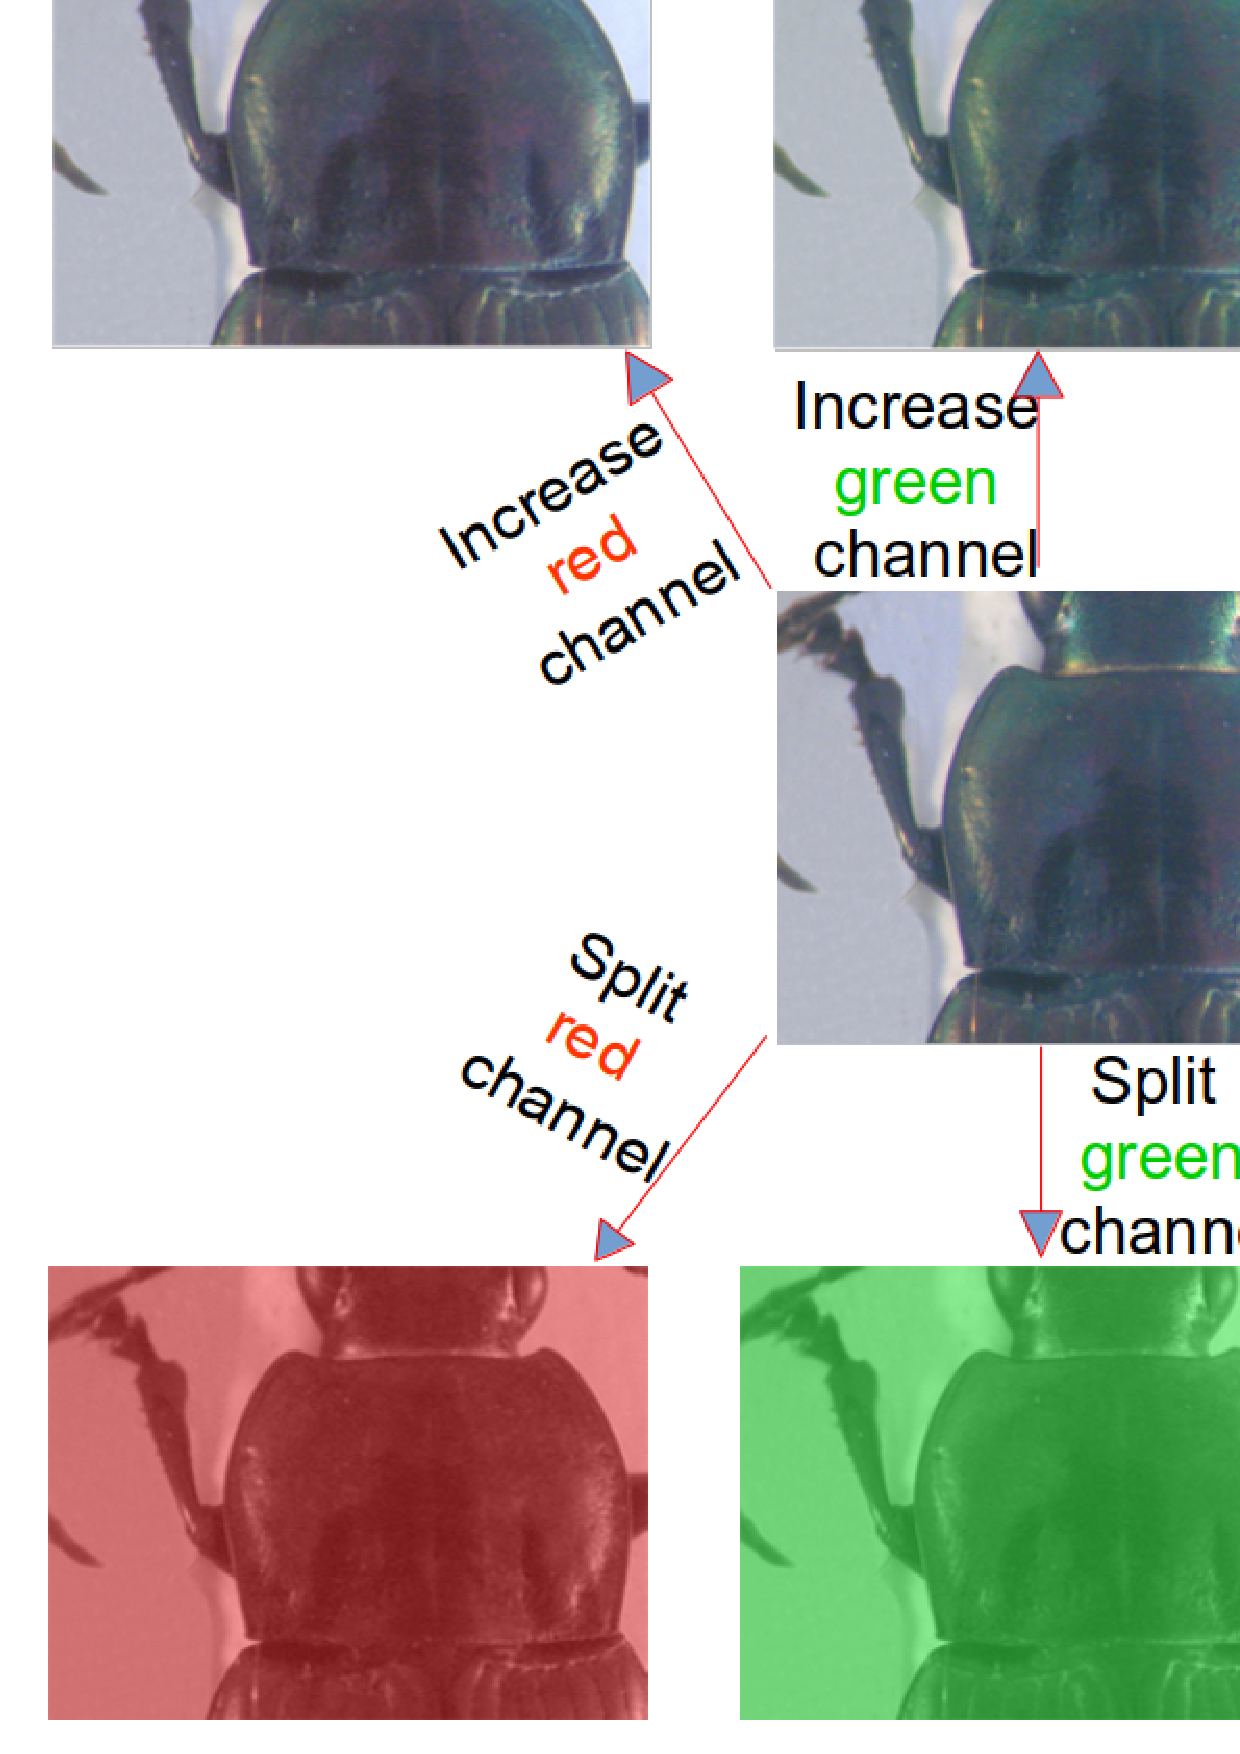
\includegraphics[width=.7\textwidth]{images/data_aug.png}
            
            \end{block}
            
            \vfill
            
            \begin{block}{Elementary block}
            	\begin{columns}
            		\begin{column}{.54\textwidth}
            			An elementary block is consists of:
            			\begin{itemize}
            				\item A Convolutional layer
            				\item A Max-Pooling layer
            				\item A Dropout layer
            			\end{itemize}
            		\end{column}
            		\begin{column}{.45\textwidth}
            			\centering
            			\includegraphics[width=.97\textwidth]{images/elementary_block.png}
            		\end{column}
            	\end{columns}
            \end{block}
            
            \vfill
            
            \begin{block}{Network architecture}
            	\begin{center}
            		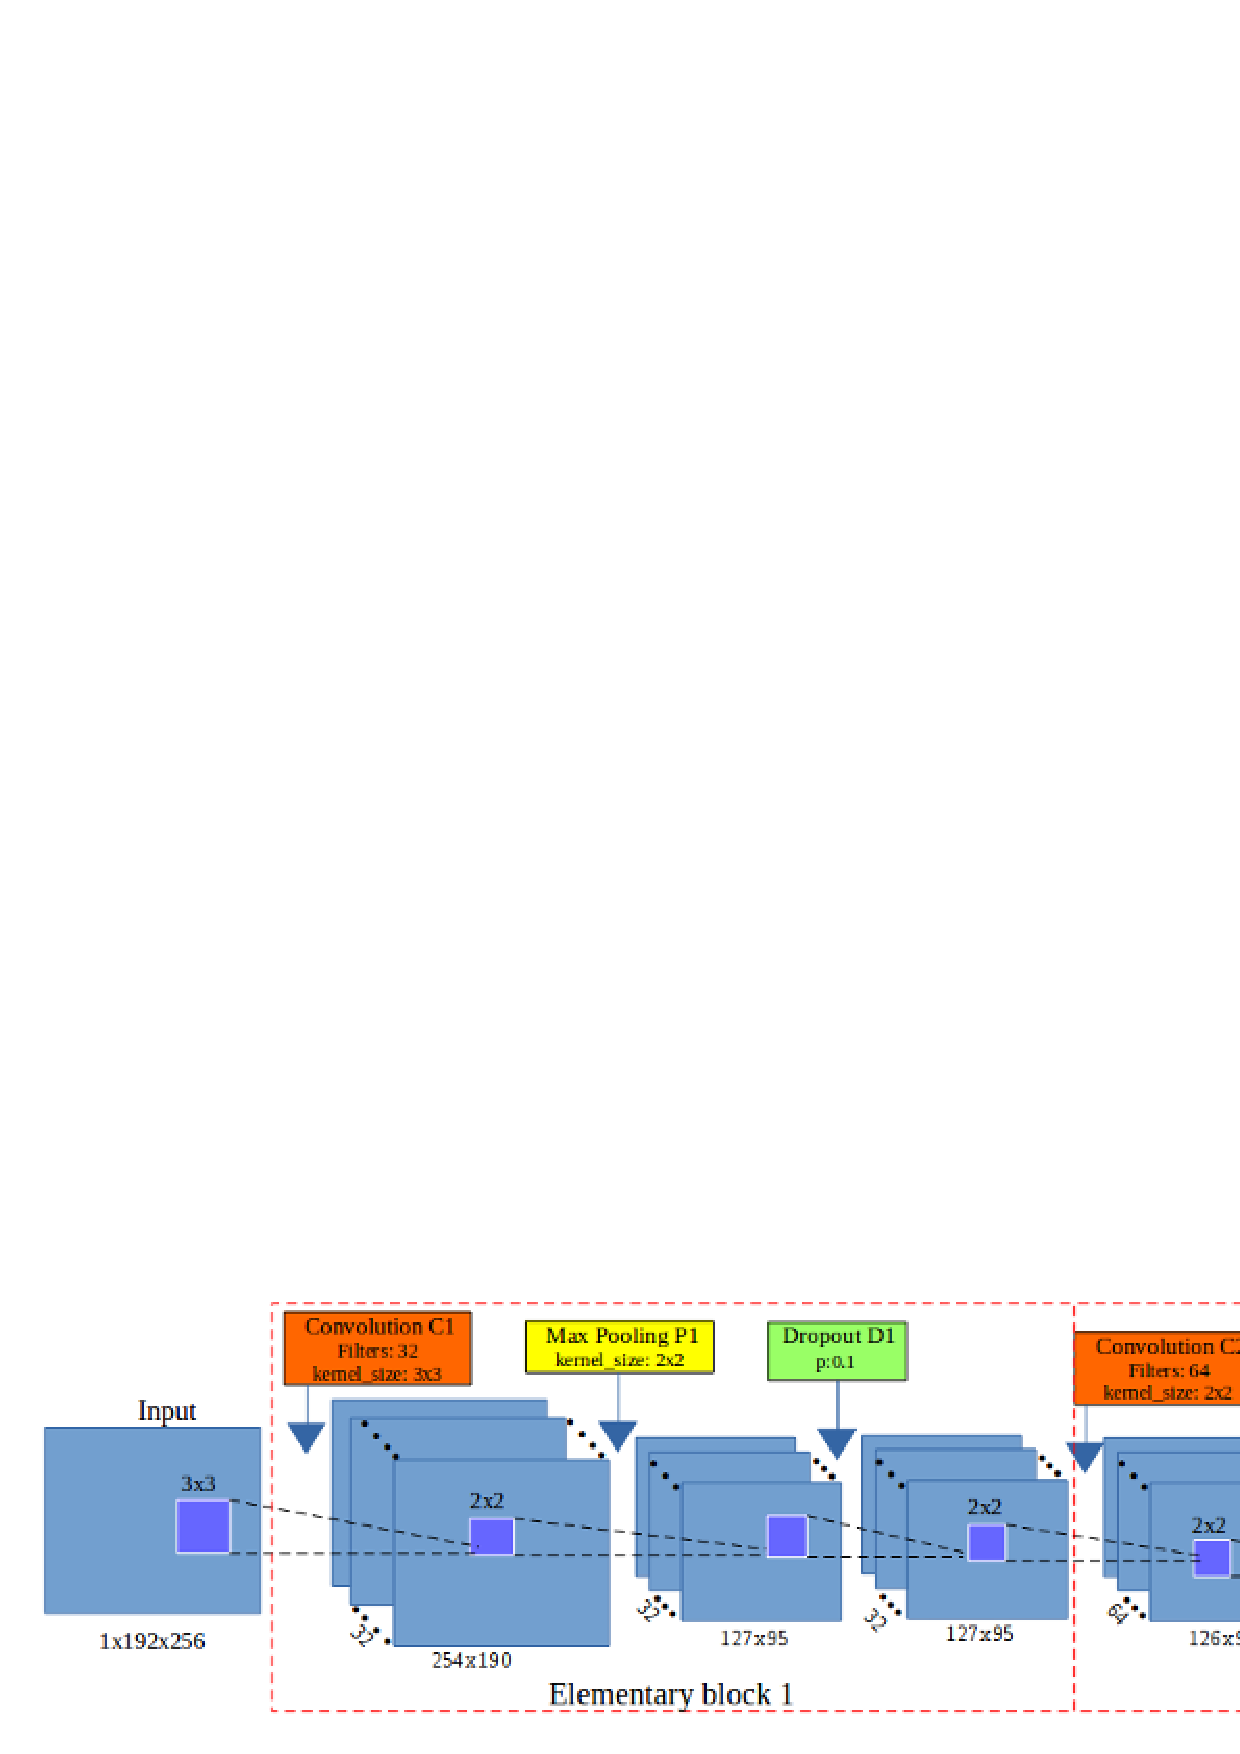
\includegraphics[width=.96\textwidth]{images/net3.png}\\
            	\end{center}
            The proposed network includes:
            \begin{itemize}
            	\item Three elementary blocks
            	\item Three fully connected layers
            	\item A Dropout layer
            \end{itemize}
            \end{block}
  
          }
        \end{minipage}
      \end{beamercolorbox}
    \end{column}
    \begin{column}{.49\textwidth}
      \begin{beamercolorbox}[center,wd=\textwidth]{postercolumn}
        \begin{minipage}[T]{.95\textwidth}
          \parbox[t][\columnheight]{\textwidth}{
            
            \begin{block}{Training curves}
            
            \centering
            
            \includegraphics[width=.925\textwidth]{sample/BP.pdf}
            
            \end{block}
            
            \vfill
            
            \begin{block}{Evaluation progresses}
            
            \centering
            
            \includegraphics[width=.8\textwidth]{sample/PS-tech.png}
            
            \end{block}
            
            \vfill
            
            \begin{block}{Conclusion}
            
            \centering
            
            Experiment: Four clients joining the system sequentially
            
            \includegraphics[width=.925\textwidth]{sample/startup.pdf}
            
            Startup delay (s) - MS-Stream (top) vs \pname (bottom)
            
            \end{block}
            
            \vfill
            
            \begin{block}{Bibliography}
            
            \begin{itemize}
            
            \item Reliability, QoE and scalability
            
            MS-Stream: Multiple-Source adaptive streaming over HTTP
            
            \item Incentive to contribute
            
            Rewarding: contributing users get a higher quality
            
            \item End-users privacy
            
            TEE (SGX): encryption, NAT and anonymity
            
            \end{itemize}
            
            \end{block}
                        
            
          }
        \end{minipage}
      \end{beamercolorbox}
    \end{column}
  \end{columns}
  \vskip1ex
\end{frame}
\end{document}

\vfill
            
            \begin{block}{MS-Stream: Multi-Source Streaming over HTTP}
            
            \centering
            
            \includegraphics[width=.925\textwidth]{sample/msstream_archi.pdf}
            
            \includegraphics[width=.925\textwidth]{sample/chunk2.pdf}
            
            \end{block}
            
            \vfill
            
            \begin{block}{Problem statement}
            
            \centering
            
            \includegraphics[width=.5\textwidth]{sample/SotA-cropped.pdf}
            
            \end{block}